\PassOptionsToPackage{unicode=true}{hyperref} % options for packages loaded elsewhere
\PassOptionsToPackage{hyphens}{url}

\documentclass[a4paper,11pt]{article}
% \usepackage[]{natbib}
\usepackage[numbers]{natbib}
\bibliographystyle{plain-fr}
\usepackage{exptech}

\usepackage{lmodern}
\usepackage{amssymb,amsmath}
  \usepackage{textcomp} % provides euro and other symbols

\usepackage{fancyhdr}


\usepackage{xcolor}
\IfFileExists{xurl.sty}{\usepackage{xurl}}{} % add URL line breaks if available
\IfFileExists{bookmark.sty}{\usepackage{bookmark}}{\usepackage{hyperref}}
\hypersetup{
  pdftitle={Jeu des pingouins à base de MCTS (Monte Carlo Tree Search) sur le navigateur en utilisant le format WebAssembly},
  pdfauthor={Clément ; Romain ; Romain ; Maxime ; Volodia ;},
  pdfborder={0 0 0},
  breaklinks=true}
\urlstyle{same}  % don't use monospace font for urls


\usepackage{color}
\usepackage{fancyvrb}
\newcommand{\VerbBar}{|}
\newcommand{\VERB}{\Verb[commandchars=\\\{\}]}
\DefineVerbatimEnvironment{Highlighting}{Verbatim}{commandchars=\\\{\}}
% Add ',fontsize=\small' for more characters per line
\newenvironment{Shaded}{}{}
\newcommand{\KeywordTok}[1]{\textbf{#1}}
\newcommand{\DataTypeTok}[1]{\underline{#1}}
\newcommand{\DecValTok}[1]{#1}
\newcommand{\BaseNTok}[1]{#1}
\newcommand{\FloatTok}[1]{#1}
\newcommand{\ConstantTok}[1]{#1}
\newcommand{\CharTok}[1]{#1}
\newcommand{\SpecialCharTok}[1]{#1}
\newcommand{\StringTok}[1]{#1}
\newcommand{\VerbatimStringTok}[1]{#1}
\newcommand{\SpecialStringTok}[1]{#1}
\newcommand{\ImportTok}[1]{#1}
\newcommand{\CommentTok}[1]{\textit{#1}}
\newcommand{\DocumentationTok}[1]{\textit{#1}}
\newcommand{\AnnotationTok}[1]{\textit{#1}}
\newcommand{\CommentVarTok}[1]{\textit{#1}}
\newcommand{\OtherTok}[1]{#1}
\newcommand{\FunctionTok}[1]{#1}
\newcommand{\VariableTok}[1]{#1}
\newcommand{\ControlFlowTok}[1]{\textbf{#1}}
\newcommand{\OperatorTok}[1]{#1}
\newcommand{\BuiltInTok}[1]{#1}
\newcommand{\ExtensionTok}[1]{#1}
\newcommand{\PreprocessorTok}[1]{\textbf{#1}}
\newcommand{\AttributeTok}[1]{#1}
\newcommand{\RegionMarkerTok}[1]{#1}
\newcommand{\InformationTok}[1]{\textit{#1}}
\newcommand{\WarningTok}[1]{\textit{#1}}
\newcommand{\AlertTok}[1]{\textbf{#1}}
\newcommand{\ErrorTok}[1]{\textbf{#1}}
\newcommand{\NormalTok}[1]{#1}


\usepackage{graphicx,grffile}
\makeatletter
\def\maxwidth{\ifdim\Gin@nat@width>\linewidth\linewidth\else\Gin@nat@width\fi}
\def\maxheight{\ifdim\Gin@nat@height>\textheight\textheight\else\Gin@nat@height\fi}
\makeatother
% Scale images if necessary, so that they will not overflow the page
% margins by default, and it is still possible to overwrite the defaults
% using explicit options in \includegraphics[width, height, ...]{}
\setkeys{Gin}{width=\maxwidth,height=\maxheight,keepaspectratio}

% Make links footnotes instead of hotlinks:
\DeclareRobustCommand{\href}[2]{#2\footnote{\url{#1}}}


\setlength{\emergencystretch}{3em}  % prevent overfull lines
\providecommand{\tightlist}{%
  \setlength{\itemsep}{0pt}\setlength{\parskip}{0pt}}

% 
% set default figure placement to htbp
\makeatletter
\def\fps@figure{htbp}
\makeatother


\title{\textbf{Jeu des pingouins à base de MCTS (\emph{Monte Carlo Tree Search}) sur le
navigateur en utilisant le format \texttt{WebAssembly}}}
\author{Clément \textsc{Chavanon} \and Romain \textsc{Hu} \and Romain \textsc{Hubert} \and Maxime \textsc{Grimaud} \and Volodia \textsc{Parol-Guarino} \and 
 \\ Encadrant : Pascal \textsc{Garcia}}

% \author{Francesco \textsc{Bariatti} \and Adrien \textsc{Gasté} \and Mikael \textsc{Le} \and Romain \textsc{Lebouc}
%         \\
%         Encadrant : Pascal \textsc{Garcia}}

\date{2019-2020}

\begin{document}
\maketitle
\begin{abstract}
Créer de toutes pièces une Intelligence Artificielle (IA) sur le jeu des
pingouins. Ce jeu est un jeu de stratégie sur plateau, sa principale
caractéristique vient de ses cases hexagonales. De plus ce jeu réagit
très bien lorsque soumis à une IA de type \emph{Monte-Carlo Tree
Search}, que nous avons codé. Le second défi de ce projet est également
sa plateforme cible : exécuter le code de l'interface et de l'IA dans un
navigateur moderne. Pour cela nous utilisons \texttt{Emscripten} qui
nous permet de compiler notre IA en \texttt{WebAssembly} et d'atteindre
des performances proches du natif. Quant au \emph{frontend}, c'est une
application classique \texttt{Angular}.

\end{abstract}

\section*{Introduction}\label{introduction}
\addcontentsline{toc}{section}{Introduction}

``Pingouins'' est un jeu de stratégie et de plateau sur lequel
s'affrontent 2 à 4 joueurs. Le plateau contient 60 cases hexagonales qui
comportent 1 à 3 poissons.

En début de partie, chaque joueur place un certain nombre de pingouins
(de 2 à 4 suivant le nombre de joueurs) sur le plateau. A chaque tour,
le joueur doit, si possible, bouger l'un de ses pingouins. Les
déplacements autorisés se font en ligne droite suivant les 6 faces de la
case hexagonale sur laquelle se trouve le pingouin. Il ne peut passer
par-dessus des trous ou au-dessus d'autres pingouins, peu importe qu'ils
appartiennent ou non au même joueur. Une fois le mouvement achevé, la
case de départ est retirée du plateau. Le joueur peut alors incrémenter
son score du nombre de poissons qu'il y avait sur cette case.

Le jeu se termine lorsque plus aucun pingouin ne peut se déplacer. Le
joueur avec le plus de points (poissons) remporte la partie.

\section{Sujet}\label{sujet}

Le sujet portait sur l'implémentation de ce jeu dans un environnement
Web, en utilisant le nouveau standard \texttt{WebAssembly}. Les sources
du projet sont compilées avec \texttt{Emscripten} qui permet de coder en
\texttt{c++} pour la partie technique. L'interface devait se faire avec
les bibliothèques \emph{Simple DirectMedia Layer}.

\subsection{Récapitulatif}\label{ruxe9capitulatif}

Afin de tester la faisabilité et les différentes technologies, nous
avons décidé de procéder à la création de l'algorithme de façon
abstraite et de tester avec un jeu simple et facilement implémentable :
le morpion (servant alors de \emph{Preuve de Concept} - PdC). Pour la
partie graphique nous avions simplement codé en JavaScript pur. Pour la
suite du projet, pour faciliter le développement de la partie front-end,
nous avons décidé de choisir : \texttt{Angular}. Sur la PdC avions testé
une autre technologie pour gérer le graphisme du jeu : \texttt{PixiJS}.
Cependant, plus tard, cela ne s'est pas avéré satisfaisant pour notre
utilisation. En effet \texttt{PixiJS} nécessite une gestion asynchrone
de son canvas, son intégration dans une application \texttt{Angular}
doit donc se faire dans une zone indépendante, le lien avec le
\texttt{WebAssembly} devenait alors trop complexe.

\subsection{Précédemment}\label{pruxe9cuxe9demment}

Ce projet n'est pas nouveau. Une précédente équipe y a déjà passé de
nombreuses heures. Cependant, afin de simplifier notre travail il a été
décidé de tout refaire, y compris le MCTS dont le code leur avait été
donné déjà optimisé. En effet, notre technologie étant récente, la
parallélisation de l'algorithme, par exemple, pouvait s'avérer plus
compliquée à porter en \texttt{WebAssembly} qu'à réécrire.

\subsection{Objectif}\label{objectif}

Nous nous sommes principalement concentrés sur le fonctionnement correct
de tout le projet et pas seulement de l'algorithme et du jeu. C'est pour
cela que nous avons choisi de présenter un résultat plus correct
qu'optimal (par exemple nous n'avons pas utilisé de représentation en
\emph{bitboards}, comme l'ont fait nos prédécesseurs, de même qu'ils
n'ont pas eu l'algorithme à gérer).

\subsection{Répartition}\label{ruxe9partition}

Pour mener à bien notre projet, les différentes tâches ont été réparties
au sein des membres du groupe. Deux équipes ont été créées :

\begin{itemize}
\tightlist
\item
  Volodia et Romain Hubert pour la création du moteur du jeu en
  \texttt{c++} et optimisation du code (multithreading)
\item
  Maxime, Romain Hu et Clément pour la création de l'interface Web et
  préparation du lien entre le moteur et la partie graphique
\end{itemize}

Finalement, la partie qui consistait à permettre de transporter le jeu
codé en \texttt{c++} vers le navigateur a été faite par les membres des
deux équipes (cf Bindings MCTS).

\section[Réalisation ]{\texorpdfstring{Réalisation \footnote{Toutes nos
  sources sont disponibles \citep{repo_git}. Nous avons également une
  démonstration en ligne \citep{repo_demo}.}}{Réalisation }}\label{ruxe9alisation-realisation}

\subsection{Environnement de
développement}\label{environnement-de-duxe9veloppement}

Devant la variété d'OS utilisés au cours de cette année par les membres
de notre équipe et le fait que nous allions développer un stack
technique peu commun en \texttt{c++} nous avons décidé de ``simplifier''
notre développement en utilisant les dernières fonctionnalités de VSCode
et en utilisant le développement dans un \emph{container} Docker. Cela
permet au projet d'être extrêmement portable et d'être fonctionnel chez
n'importe quel développeur !

Et en bonus nous avons réalisé ce rapport en \texttt{Markdown} afin
qu'il soit facilement visible sur notre \emph{repository}.

\subsection{Représentation du jeu}\label{repruxe9sentation-du-jeu}

Notre encadrant nous a indiqué au tout début du projet un guide de
méthodologies complet sur les plateaux hexagonaux et leurs
représentations en informatique \citep{patel_blobs_2019}. En se basant
sur ce guide et sur la forme rectangulaire de notre plateau, nous avons
choisi une représentation en mémoire avec un conteneur associatif sous
forme de table de hachage :
\VERB|\BuiltInTok{std::}\NormalTok{unordered_map}|, d'une part afin
d'obtenir une complexité en temps en \(O(1)\) moyen et pas de
\(O(log(n))\) moyen avec les classiques, soit avec un conteneur
associatif basé sur des arbres équilibrés :
\VERB|\BuiltInTok{std::}\NormalTok{map}|. La représentation de la grille
hexagonale sous forme rectangulaire crée des parties non utilisées dans
le tableau \citep[voir la section \emph{map storage}]{patel_blobs_2019}.

\subsection{Points sensibles}\label{points-sensibles}

Utiliser un algorithme tel que le MCTS implique que la vitesse et
l'efficacité de ce dernier vont grandement être impactés par la
représentation. Pour le MCTS, deux méthodes de la représentation du jeu
ont un impact très important pour le niveau de l'intelligence
artificielle que l'on obtient :

\begin{itemize}
\tightlist
\item
  la méthode servant à donner tous les cas disponibles pour un joueur,
  qui doit en effet analyser quelles routes sont possibles et jusqu'à
  quel endroit\footnote{Un pingouin peut être bloqué par un trou dans le
    plateau ou un autre pingouin.};
\item
  la méthode servant à donner l'état du jeu (aussi utilisée pour
  connaître le joueur suivant \footnote{Il arrive qu'un joueur soit
    bloqué et qu'attendre son tour ne serve à rien, son adversaire peut
    lui continuer à récolter tous les points.}) qui doit vérifier s'il
  est encore possible pour un joueur de bouger \footnote{Un pingouin
    peut être bloqué par un trou dans le plateau ou un autre pingouin.}.
\end{itemize}

Une passe d'optimisation a déjà été réalisée sur la deuxième méthode qui
reposait à la base sur la première (dans un effort d'obtenir le plus
vite une démo fonctionnelle afin de déboguer des points plus vitaux).
Cependant le temps manque pour faire plus, notamment nos prédécesseurs
ont eu le temps\footnote{L'équipe précédente n'a pas eu à faire le MCTS
  et avait directement une interface connectant la représentation avec
  cet algorithme, sur laquelle nous avons dû faire quelques ajustements
  après avoir développé la représentation du jeu des pingouins. Nous
  faisons allusion ici à une différence entre le pion et le joueur : un
  joueur peut posséder plusieurs pions et ceci n'était pas une
  contrainte sur notre première phase de tests avec un morpion\ldots{}}
de vraiment attaquer le vif de l'optimisation, notamment avec les
\emph{bitboards}, qui leur ont permis une belle différence de
performance (sans compter ici le fait que nous développons pour le web).

\section{MCTS}\label{mcts}

\subsection{Principe}\label{principe}

Le \emph{Monte Carlo Tree Search} (ou MCTS) est un algorithme de
recherche heuristique. C'est un algorithme qui explore l'arbre des
possibles. Au fur et à mesure que l'algorithme se déroule, cet arbre
grandit. Il essaye d'explorer toutes les parties possibles du jeu, en
privilégiant les issues favorables pour lui. L'arbre est composé de
noeuds répartis sur plusieurs couches. Chaque noeud représente une
configuration, et ses enfants sont les configurations suivantes. Les
noeuds doivent aussi stocker le nombre de parties gagnantes et le nombre
total de simulations (à partir de ce noeud).

Le principe de l'algorithme est simple ; il n'y a que quatre étapes. On
commence par choisir le ``meilleur'' noeud terminal. On détermine le
meilleur noeud terminal grâce à la fonction UCT qui permet d'évaluer le
meilleur compromis entre le nombre de visites et le résultat du noeud.
Puis on crée ses enfants. Ensuite, on choisit un de ses enfants et on
simule une partie aléatoire. Enfin, on transmet ce résultat sur tous les
noeuds jusqu'à la racine.

\begin{figure}
\centering
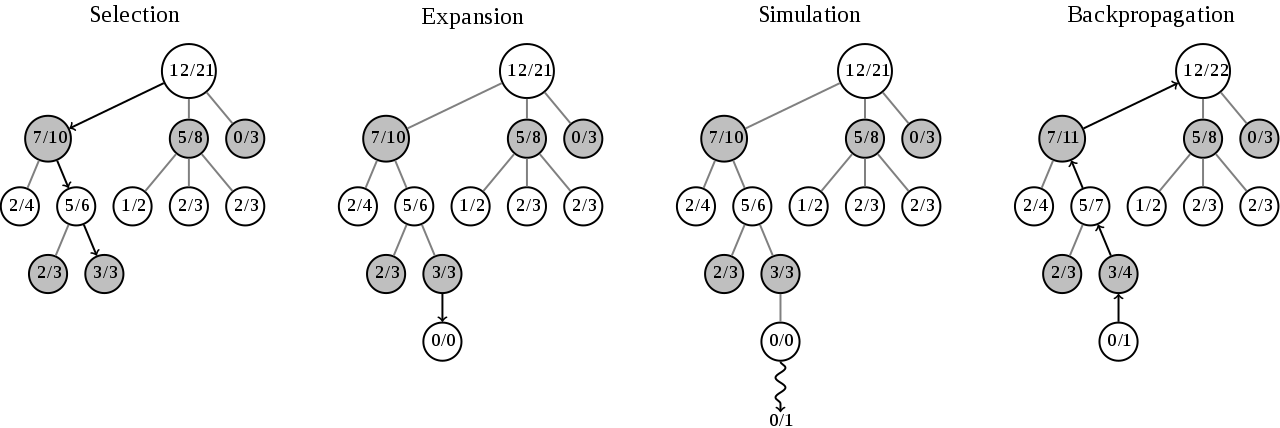
\includegraphics{mcts.png}
\caption{``Les quatre étapes du MCTS''}
\end{figure}

On répète ces 4 étapes jusqu'à ce qu'on arrête l'algorithme. Ensuite, il
nous retourne le meilleur coup à jouer, basé sur le nombre de visites
des enfants de la racine.

\subsection{Parallélisation}\label{paralluxe9lisation}

Afin d'augmenter les performances du MCTS, nous nous sommes penchés sur
le multithreading. En effet, cela nous débloque la possibilité de
simuler plusieurs parties en même temps, impliquant une augmentation du
nombre de parties simulées. Il y a différentes manières de multithreader
le MCTS; la \emph{tree parallelization}, la \emph{root parallelization}
et la \emph{leaf parallelization}. D'après cette étude
\citep{mass_par_mcts, par_mcts}, la \emph{root parallelization} semble
la meilleure puisqu'elle permet d'explorer plus d'issues que les autres
méthodes. Ainsi, cela augmente les chances de victoire du MCTS. De plus,
cette méthode est facile à implémenter. En effet, il suffit d'assigner
un arbre sur chaque thread. Les arbres sont donc développés
indépendamment entre eux, donc il y a moins de chances que l'algorithme
se bloque sur un minimum local. A la fin du temps alloué, nous mettons
en commun les arbres, uniquement la première couche pour diminuer le
temps de calcul. Ensuite, nous choisissons le meilleur coup à jouer.

Pour éviter de recréer l'arbre à chaque fois, nous avons mis en place un
système de déplacement de la racine à un de ses enfants, gardant ainsi
le sous-arbre de l'enfant.

\section{Interface graphique}\label{interface-graphique}

Pour offrir une expérience de jeu optimale, et afin d'exporter le jeu
sur un navigateur, nous avons dû mettre en place une interface graphique
pour notre jeu. Avec les contraintes de temps et les contraintes
techniques, nous avons été amenés à faire des choix aux niveaux des
technologies utilisées et des méthodes d'implémentation afin de pouvoir
produire rapidement une interface utilisable.

\subsection{\texorpdfstring{\texttt{Angular} \&
\texttt{Ionic}}{Angular \& Ionic}}\label{angular-ionic}

Afin de mettre en place, un code solide et rapidement exploitable, nous
voulions impérativement utiliser \texttt{Typescript}, pour réaliser le
moteur de jeu côté graphisme. En effet, son contrôle de typage est un
véritable plus, par rapport à notre preuve de concept, où le moteur du
morpion était en \texttt{Javascript}. D'autre part, nous voulions
construire une architecture de site Web plus globale qui viendrait
englober la partie véritablement jouable. Afin de mettre en place cette
architecture web sur pied au plus vite, nous nous avons décidé
d'utiliser \texttt{Angular}.

Pour mettre en place la charte graphique de notre application, nous nous
sommes tournés vers le framework \texttt{Ionic\ 4}, sorti récemment, qui
offre aux développeurs des thèmes pré-conçus et des composants
adaptatifs. Basé sur \texttt{Angular}, il s'intègre donc parfaitement
dans notre projet.

\subsection{Organisation de
l'application}\label{organisation-de-lapplication}

Dans sa version finale notre application se compose des pages
principales suivantes :

\begin{itemize}
\tightlist
\item
  une page d'accueil présentant le projet,
\item
  une page avec le jeu en lui même,
\item
  une page de présentation pour les membres de l'équipe,
\item
  et une page pour les crédits.
\end{itemize}

\begin{figure}
\centering
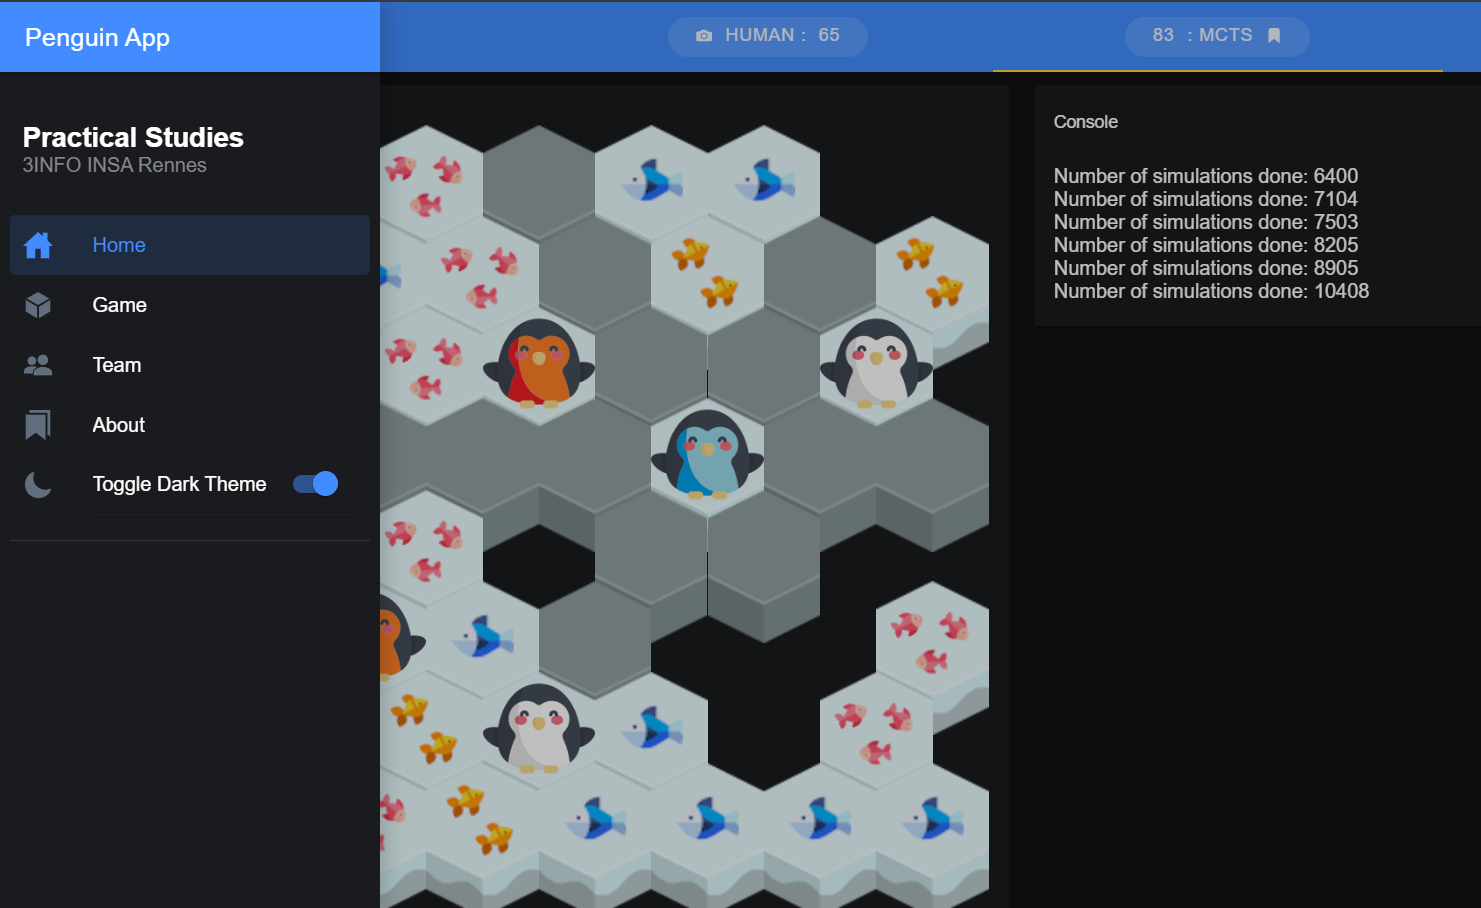
\includegraphics{penguinApp.png}
\caption{``Aperçu interface graphique''}
\end{figure}

Cette dernière permet, en plus de mettre à disposition le jeu des
pingouins dans un navigateur web, de présenter le projet dans sa
globalité, ainsi que les membres de l'équipe ayant participé à sa
réalisation. L'ensemble du rendu graphique est défini par un ensemble de
composants venant s'incruster dans des \emph{pages Ionic}. La gestion et
la levée d'évènement se fait conformément au standart \emph{Angular}, et
par un jeu de double bindings dans la hiérarchie des composants.

\begin{Shaded}
\begin{Highlighting}[numbers=left,,firstnumber=0,]
\CommentTok{// Organisation de penguinApp}
\NormalTok{|-> pages}
\NormalTok{    |-> home}
\NormalTok{    |-> game}
\NormalTok{        |-> board}
\NormalTok{            |-> hex}
\NormalTok{            |-> penguin}
\NormalTok{            |-> models}
\NormalTok{        |-> control}
\NormalTok{        |-> console}
\NormalTok{        |-> info}
\NormalTok{     |-> team}
\NormalTok{     |-> about}
\end{Highlighting}
\end{Shaded}

Durant nos recherches dans les différentes possibilités que pouvaient
nous offrir \emph{Ionic}, nous avons mis en place la possibilité
d'accéder à une deuxième charte graphique, définissant le
\texttt{Dark\ Theme}.

\subsection{Automates finis}\label{automates-finis}

Que ce soit pour l'application entière, ou le jeu en particuler il a
fallu mettre en place des automates finis (\emph{Finite-State Machine}),
afin de gérer le flot de contrôle, et contenir les actions possibles en
fonction de l'état d'avencement.

Le flot de contrôle est contenu par 2 machines à états :

\begin{itemize}
\tightlist
\item
  une pour l'application globale (apparition des différents composants
  en fonction des interactions avec l'utilisateur)
\item
  une deuxième pour gérer exclusivement le jeu
\end{itemize}

Pour mettre en place, ces automates finis, nous avons utilisé la
librairie \emph{Typescript} \texttt{+xstate}, permettant de mettre en
place rapidement des automates sous le jormat \emph{JSON}. Cette
dernière offre aussi un système de visualisation des machines.

\begin{figure}
\centering
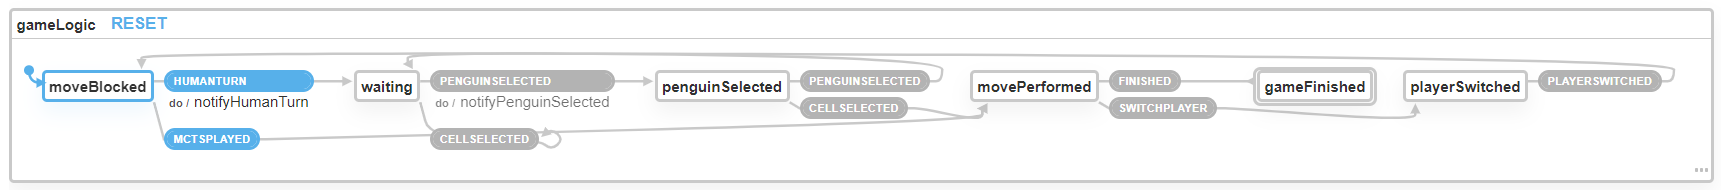
\includegraphics{gameMachine.png}
\caption{``Aperçu Automate fini du jeu''}
\end{figure}

L'Automate du jeu permet de dérouler la logique du jeu des pingouins, en
limitant les interactions en fonction du joueur qui doit jouer. Le
passage d'un état à un autre se fait par le déclenchement d'une action
pré-enregistrée, souvent cette dernière est associée à un événement sur
un composants \emph{Ionic}. La progression dans le jeu se fait donc
complètement indépendamment de l'application dans laquelle il est
intégré.

Cette manipulation d'état et d'événements permet d'offrir à
l'utilisateur une intéraction agréable et visuelle avec le plateau de
jeu.

\section{Liens entres toutes les
parties}\label{liens-entres-toutes-les-parties}

Il faut maintenant faire le lien entre l'interface graphique et le cœur
du jeu. Il existe plusieurs niveaux de difficulté pour réaliser ces
liens. Le plus simple nous l'avons utilisé lors de notre preuve de
concept avec le morpion. Elle consiste à marquer les fonctions à
exporter directement dans la commande de compilation et est adaptée pour
une petite quantité de fonctions. Cependant, le passage à l'échelle ne
se fait pas bien, c'est pour cela que nous avons utilisé la seconde
méthode : \emph{Embind} \citep{embind}. Elle se traduit pour
l'utilisateur en de simples lignes d'export de méthodes dans un
préprocesseur. Les seules difficultés peuvent venir des \emph{templates}
en \texttt{c++} qui peuvent faire grossir le code, mais un préprocesseur
adapté suffit à limiter cela et de l'organisation générale du projet.
C'est-à-dire que suivant où l'on situe ces lignes de lien, on peut avoir
du mal à savoir quels classes sont concernées, c'est pour cela qu'en
nous inspirant de \texttt{Angular} nous avons un ficher avec l'extension
\texttt{*.bind.cpp} qui reprend toutes les fonctions exportées dans le
dossier courant et permet ainsi d'avoir très peu de méthodes à écrire
juste pour les liens. Le compilateur se charge alors de réaliser les
liens automatiquement (et mêmes des pointeurs\footnote{Il existe les
  pointeurs intelligents en c++, seulement notre première utilisation de
  ces derniers a été d'utiliser la version
  \VERB|\BuiltInTok{std::}\NormalTok{shared_pointers}| à la première
  occasion. Devant notre ignorance nous nous sommes rabattus sur le
  classique des pointeurs \texttt{C}. Si nous avions continué nous
  aurions certainement abusé des pointeurs \texttt{shared} et fini par
  perdre massivement en performance et en mémoire, surtout que nous
  avions déjà en tête de multithreader notre application. Nous ne
  parlons que des \texttt{shared\_pointers} puisque nous ne connaissions
  pas réellement les mécanismes de \emph{ownership} des
  \texttt{unique\_pointers}.} !). De plus la clarté gagnée par cette
structure permet aussi de continuer à garder deux plateformes pour
développer : le Web et Linux pour avoir accès à l'éventail d'outils de
débogage existants. Un exemple d'un tel code est le suivant :

\begin{Shaded}
\begin{Highlighting}[numbers=left,,firstnumber=0,]
\NormalTok{...}
    \CommentTok{// Only target Emscripten compilation (auto-generated flag)}
\PreprocessorTok{#ifdef __EMSCRIPTEN__}
\NormalTok{...}
\KeywordTok{using} \KeywordTok{namespace}\NormalTok{ emscripten;}

\CommentTok{// Binding code}
\NormalTok{EMSCRIPTEN_BINDINGS(mcts_bind)}
\NormalTok{\{}
    \CommentTok{// Here exporting a c style structure with a field}
\NormalTok{    value_object<MCTSConstraints>(}\StringTok{"MCTSConstraints"}\NormalTok{)}
\NormalTok{        .field(}\StringTok{"time"}\NormalTok{, &MCTSConstraints::time);}

    \CommentTok{// It is a bit more complex to export a template,}
    \CommentTok{// especially if we want to take fully advantage }
    \CommentTok{// of why they were made in the first place :}
    \CommentTok{// multiple types}
\PreprocessorTok{#define __MCTS_BIND__(name_prefix, MCTSPlayer, AbstractGame)                               }\NormalTok{\textbackslash{}}
\PreprocessorTok{    class_<MCTSPlayer>(name_prefix "_MCTSPlayer")                                          }\NormalTok{\textbackslash{}}
\PreprocessorTok{        .constructor<AbstractGame *const &, const MCTSConstraints &>}
\NormalTok{                                            (allow_raw_pointers()) \textbackslash{}}
\NormalTok{        .function(}\StringTok{"bestMove"}\NormalTok{, &MCTSPlayer::bestMove) }
    \CommentTok{// We need to define the types (by clarity + }
    \CommentTok{//                  limitation of the preprocessors)}
    \KeywordTok{typedef}\NormalTok{ MCTSPlayer< ... > }\DataTypeTok{penguin_mcts_player_t}\NormalTok{;}
    \KeywordTok{typedef}\NormalTok{ game::AbstractGame< ... > }\DataTypeTok{penguin_game_t}\NormalTok{;}
    \CommentTok{// We use it for the penguin game,}
    \CommentTok{// but it is as easy to export for the tic tac toe demo}
\NormalTok{    __MCTS_BIND__(}\StringTok{"penguin"}\NormalTok{, }\DataTypeTok{penguin_mcts_player_t}\NormalTok{, }\DataTypeTok{penguin_game_t}\NormalTok{);}
\NormalTok{\}}

\PreprocessorTok{#endif}
\end{Highlighting}
\end{Shaded}

Notre second défi a été de lier la version parallélisée de notre
programme avec \texttt{pthreads}\citep{pthreads_emscripten} et
l'interface graphique. En effet, le Web a introduit sa propre version
des \emph{threads} : les \emph{WebWorkers}\footnote{Tout comme le
  \texttt{WebAssembly} les \emph{WebWorkers} ont un support encore
  limité aux versions récentes des navigateurs, pour ceux ne l'ayant pas
  désactivé pour des raisons de sécurité.}. Cependant ils possèdent leur
propre espace mémoire complètement séparé de l'application et ne
permettent qu'une communication via des types primitifs : les
\texttt{int} ou les \texttt{strings}. Il n'est donc pas aisé de
communiquer des valeurs d'instances entres ces \emph{WebWorkers}.
Heureusement pour nous, le plus gros du travail est réalisé par
\emph{Emscripten}. Néanmoins, nous avons eu un problème inacceptable :
le blocage du \emph{thread} principal de notre application lors du
développement des arbres du MCTS, l'interface ne répondait alors plus.
Pour pallier cela nous avons mis en place un mécanisme reposant sur
\emph{Asyncify} \citep{asyncify} qui permet de faire des \texttt{pause}
et \texttt{resume} dans le code \texttt{c++} exporté. Plus largement ce
module permet de rendre le code asynchrone et donc de poursuivre le
traitement des évènements tant appréciés de \emph{JavaScript} lors de
l'exécution de notre algorithme qui n'est alors plus bloquant. Le
résultat n'est pourtant pas ce que nous espérions, puisque la fonction
exécutant le MCTS ne renvoie alors plus de valeur au final. Nous avons
alors défini une fonction \emph{JavaScript} dans le code \texttt{c++},
de façon à ce que ce dernier puisse l'appeler. Cette fonction permet
alors d'émettre un événement après que la fonction \texttt{c++} ait
terminé {[}\^{}whyafterterm{]}. Cette notification permet alors à
l'interface de savoir quand récupérer la valeur de sortie et de pallier
le problème initial.

\section*{Conclusion}\label{conclusion}
\addcontentsline{toc}{section}{Conclusion}

La mise en place de ce projet a permis de mettre en évidence les
difficultés liées à la gestion de ce type de travail, notamment au
niveau de l'organisation et les échéances temporelles. Notablement, au
début nous n'avions pas les mêmes quantités de travail pour l'équipe
graphique que pour la première version du MCTS.

Les technologies utilisées étaient le second point important de ce
projet, certaines étaient déjà connues -- voire maîtrisées -- par des
membres du groupe, néanmoins la plupart se sont avérées être une totale
découverte. Il fallait donc être capable d'acquérir des connaissances
technologiques (\texttt{WebAssembly}, MCTS\_, \emph{Multithreading},
\texttt{Angular} \ldots{}) mais également dans les outils nécessaires
pour travailler dans une position peu commune (\emph{VSCode},
\texttt{Docker}, \texttt{Doxygen}, \texttt{Compodoc}) tout en
développant -- pour permettre au projet d'avancer. Finalement, le
résultat attendu par le cahier des charges a été plus qu'atteint : en
effet, nous sommes en mesure de proposer un jeu des pingouins,
implémentant une intelligence artificielle, et jouable à partir d'un
navigateur Web. Nous avons démontré la viabilité et la maturité du
\emph{WebAssembly}\footnote{un point étonnant est la possibilité
  d'allier deux géants dans leurs domaines : la versatilité du
  \texttt{JavaScript} et la puissance crue du \texttt{c++}.}, tout en se
heurtant à des obstacles -- pas impossibles à passer -- mais néanmoins
gênants pour un environnement de production. Cette expérience nous a
permis, en plus d'approfondir nos connaissances acquises au cours de
l'année, de mieux connaître le fonctionnement de chacun et d'apprendre,
en demandant conseil à notre encadrant lorsque cela devenait ardu, mais
aussi à présenter notre travail \footnote{L'exercice s'est avéré étrange
  mais encourageant.}.

Pour finir :

\begin{quote}
\emph{Laissons l'avenir dire la vérité, et évaluer chacun en fonction de
son travail et de ses accomplissements. Le présent est à eux ; le futur,
pour lequel j'ai réellement travaillé, est mien.}

-- Nikola Tesla
\end{quote}

% % \bibliography{references}
% 
\bibliography{references}

\end{document}
